\documentclass{beamer}
\setbeamercovered{transparent}
\usepackage{listings}
\usepackage[T1]{fontenc}
\usepackage{booktabs}

%% \usetheme{default}

\usetheme[pageofpages=of,% String used between the current page and the
                         % total page count.
          bullet=circle,% Use circles instead of squares for bullets.
          titleline=true,% Show a line below the frame title.
          titlepagelogo=opensuse,
          alternativetitlepage=true,% Use the fancy title page.
          ]{Torino}


\setbeamerfont{title}{series=\bfseries,size=\LARGE}
\author{Alberto Planas <aplanas@suse.de>\newline {\small openSUSE Team}}
\title{openSUSE in Numbers}
\subtitle{Basic numbers in the openSUSE project}


\AtBeginSection[]{
  \setbeamercolor{background canvas}{bg=chameleongreen3}
  \begin{frame}[plain]
    \begin{center}\begin{huge}\textcolor{white}{\secname}\end{huge}\end{center}
  \end{frame}
  \setbeamercolor{background canvas}{bg=}
}

\AtBeginSubsection[]{
  \setbeamercolor{background canvas}{bg=chameleongreen3}
  \begin{frame}[plain]
    \begin{center}\begin{huge}\textcolor{white}{\subsecname}\end{huge}\end{center}
  \end{frame}
  \setbeamercolor{background canvas}{bg=}
}


\begin{document}

\begin{frame}[t,plain]
  \titlepage
\end{frame}


\section{Downloads}

\begin{frame}{Methodology}
  \begin{itemize}
  \item Take all ISO downloads
  \item Group ISOs into products (openSUSE versions)
  \item We do not collapse by IP, so:
    \begin{itemize}
    \item every download from the same proxy, and
    \item every different product downloaded by the same user
    \item ... are counted independently
    \end{itemize}
  \item Raw data is 2Gb per day, compressed!
  \item Now 1.5Tb in BerkeleyDB queues
  \end{itemize}
\end{frame}

\begin{frame}{Daily Downloads}
  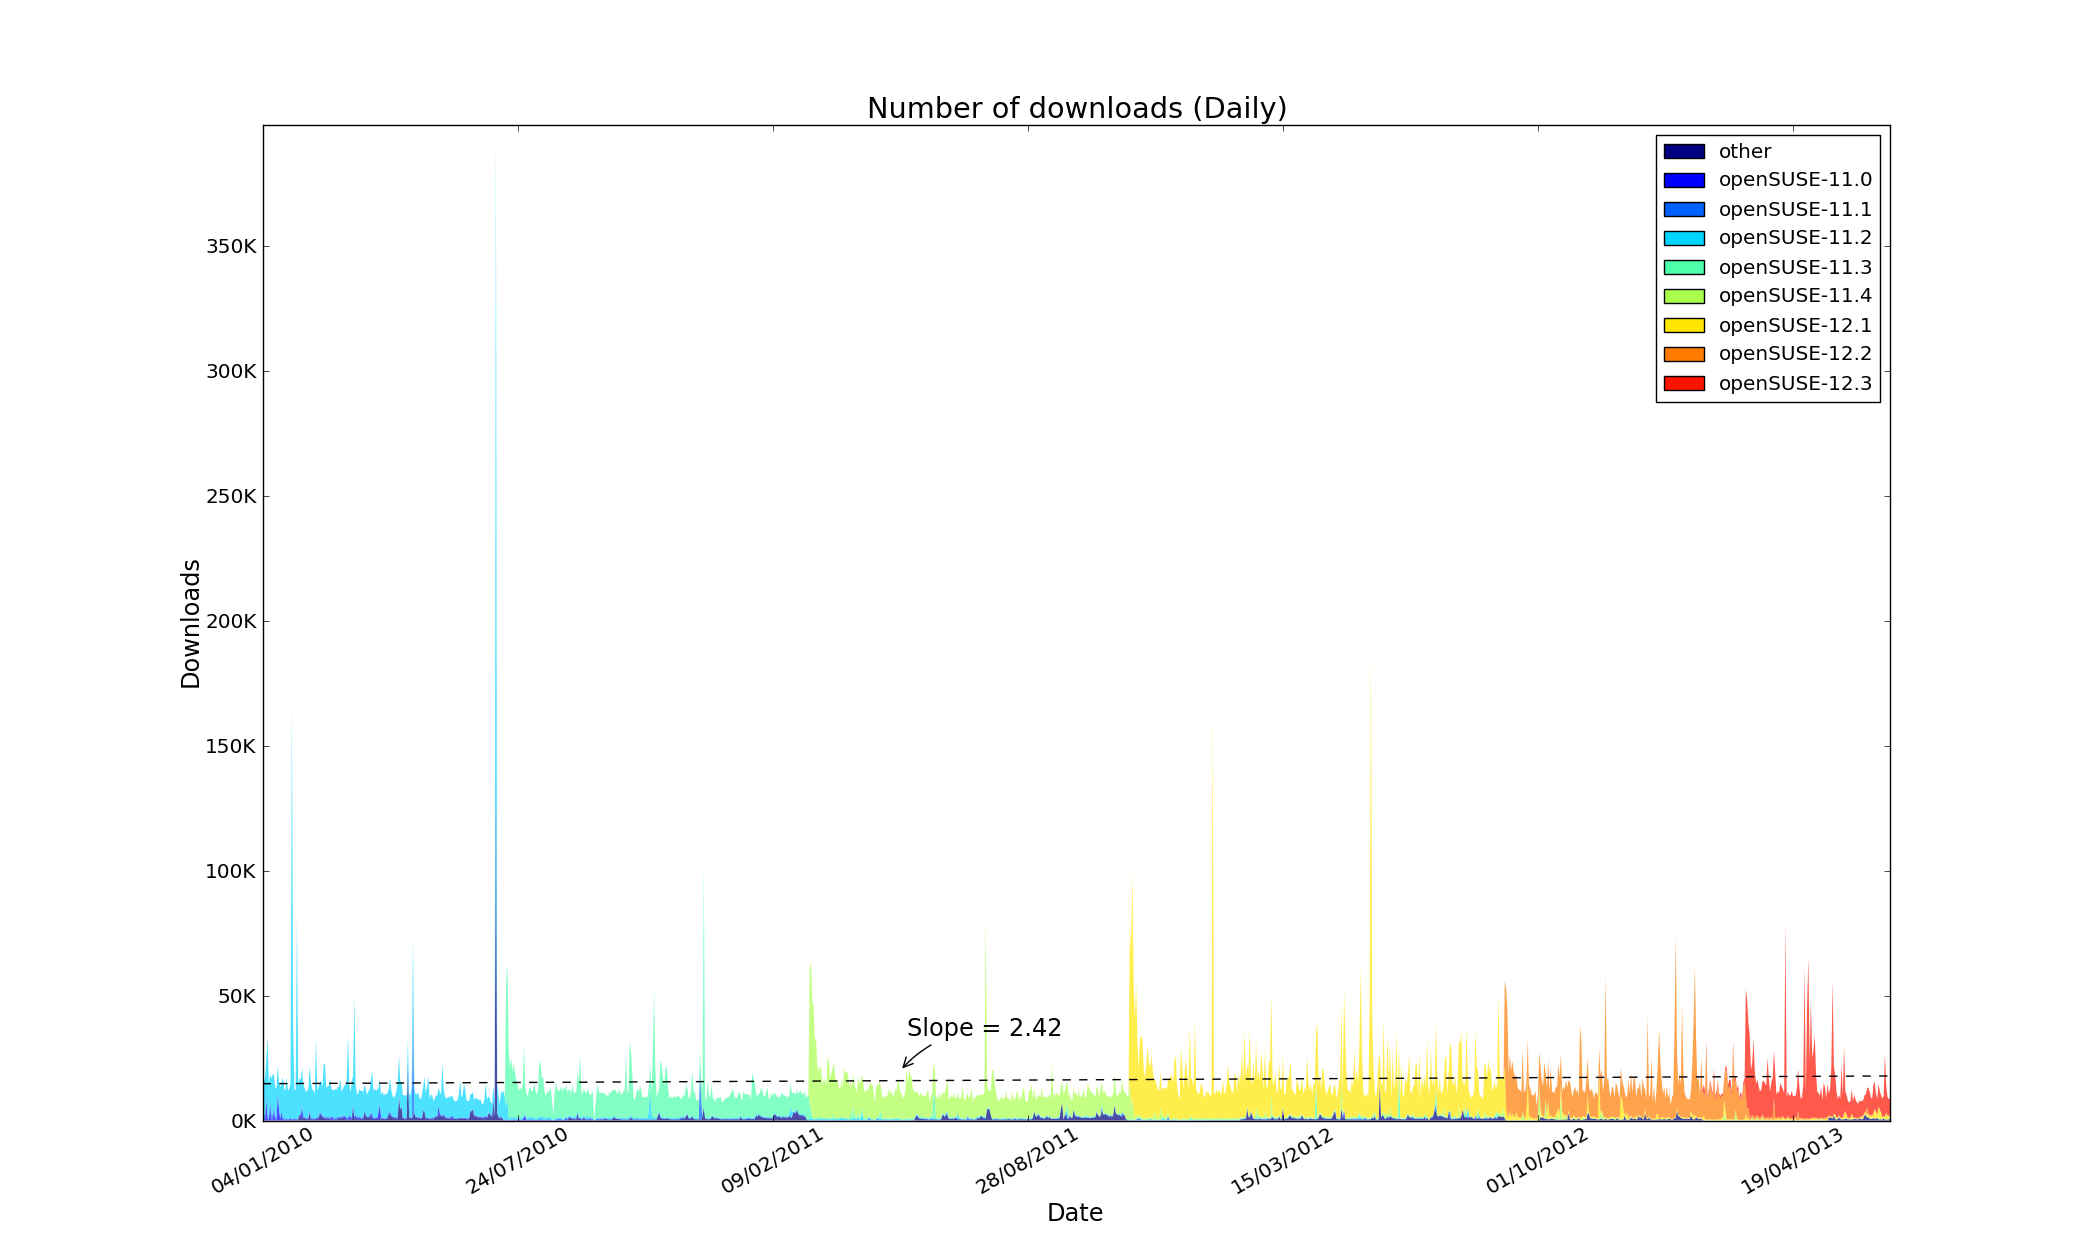
\includegraphics[height=7.2cm]{download_day}
\end{frame}

\begin{frame}{Weekly Downloads}
  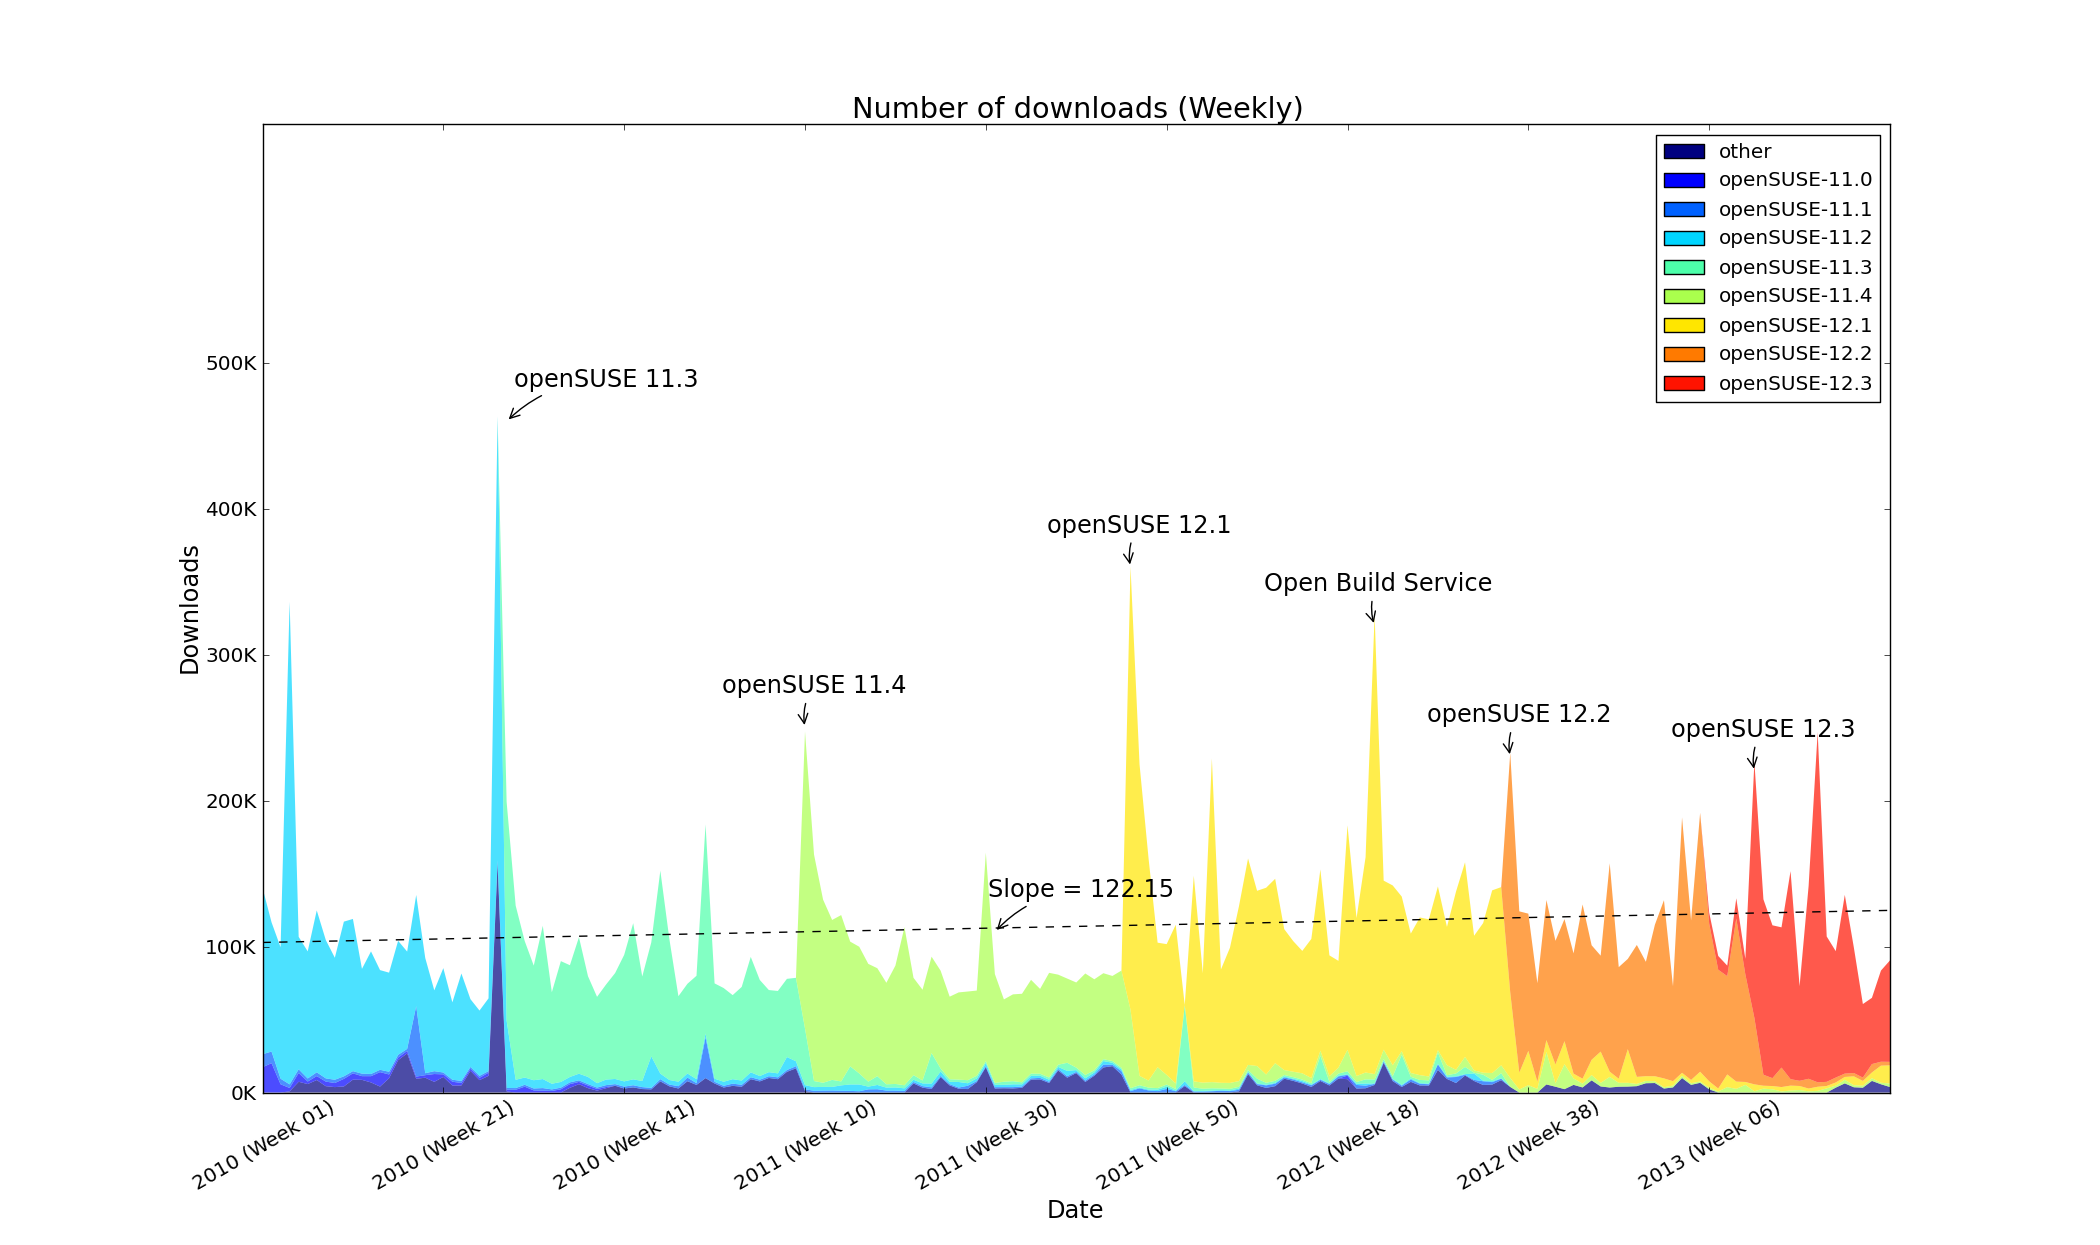
\includegraphics[height=7.2cm]{download_week}
\end{frame}

\begin{frame}{Monthly Downloads}
  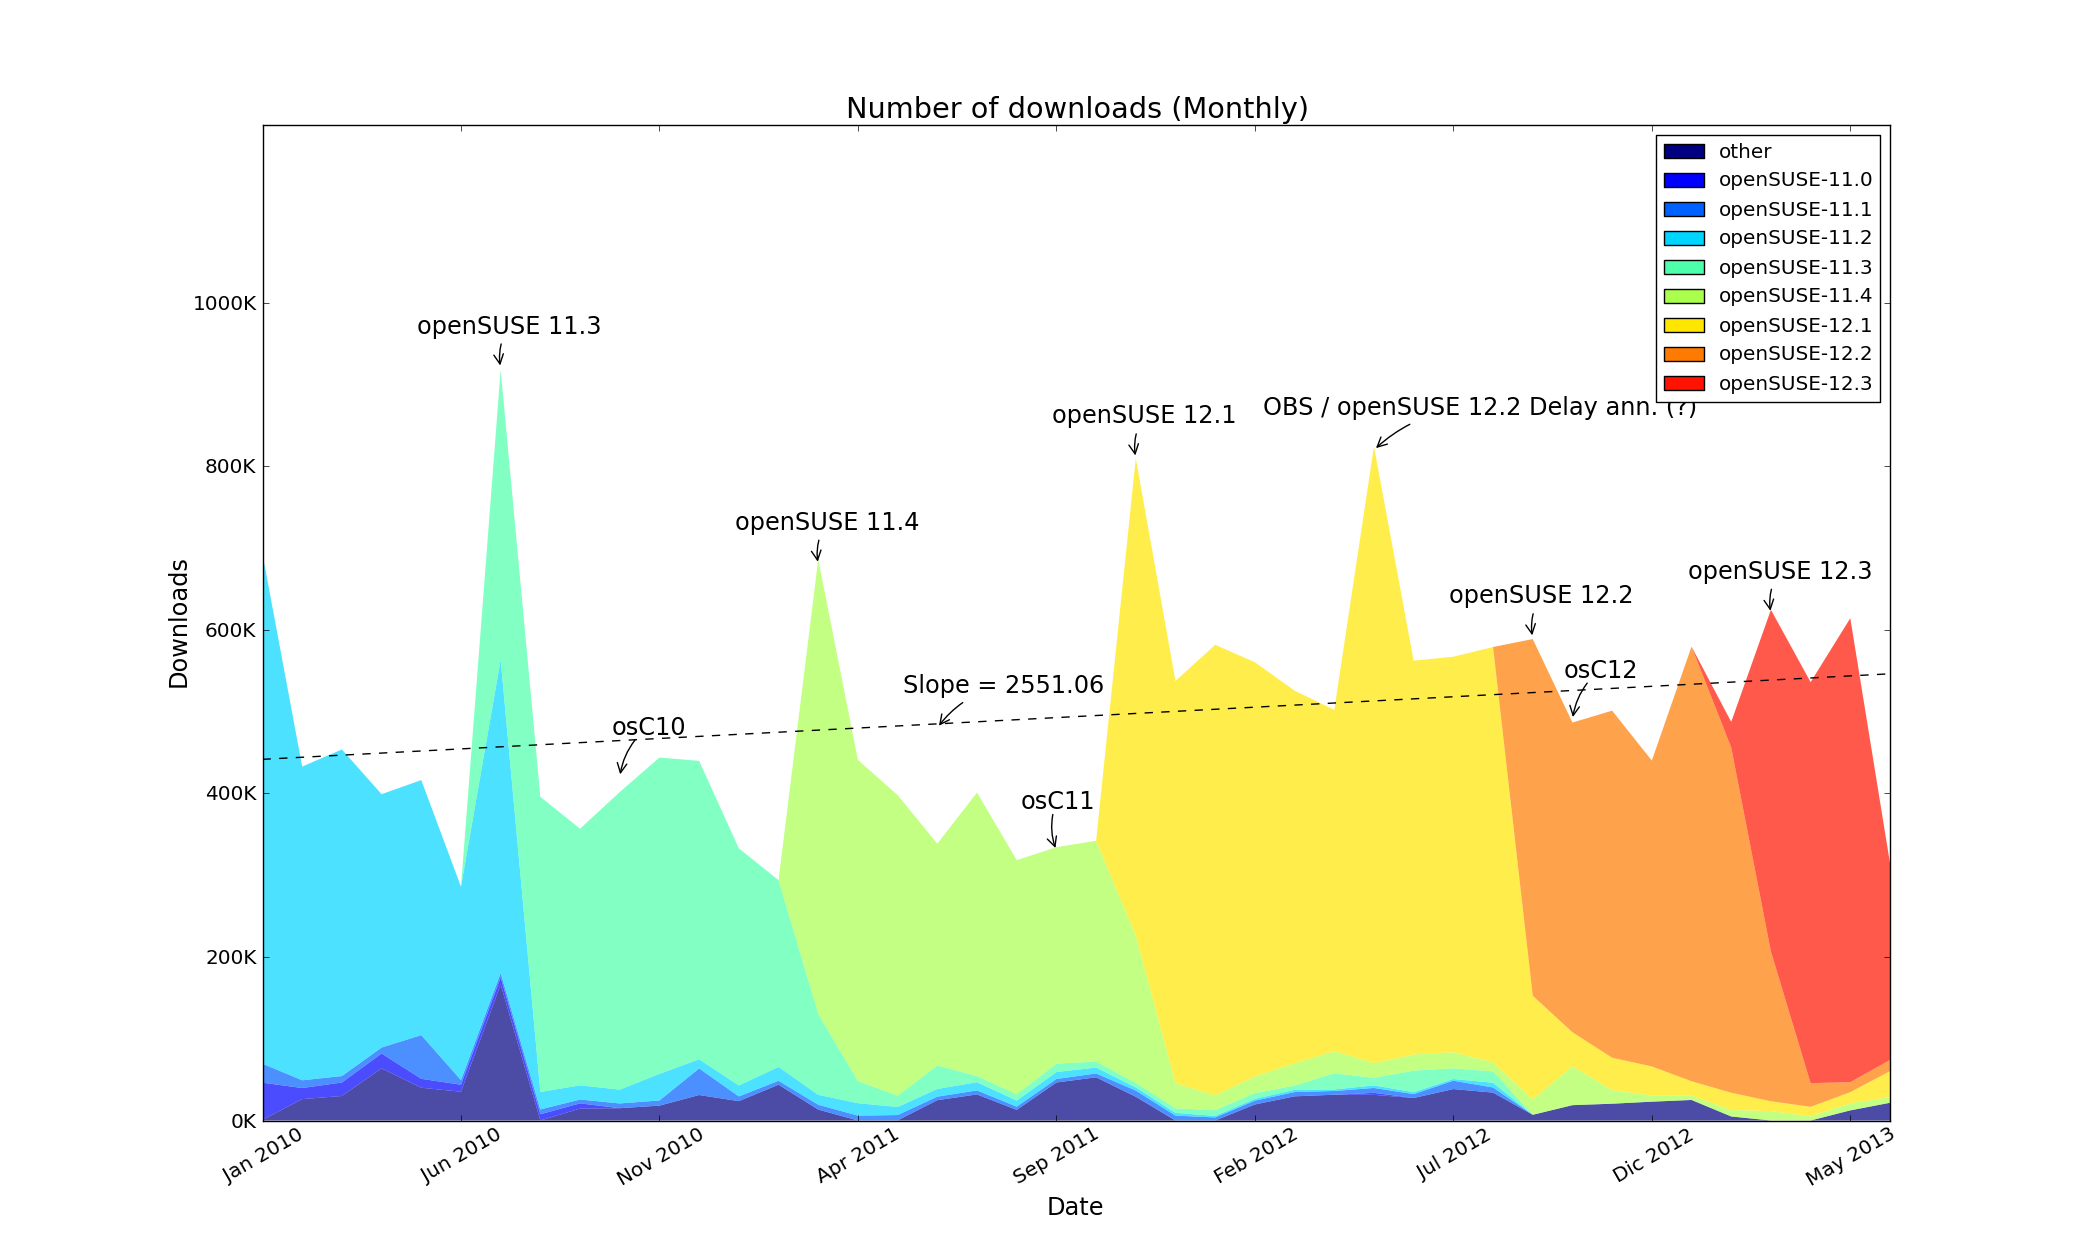
\includegraphics[height=7.2cm]{download_month}
\end{frame}

\begin{frame}{Download Model}
  \begin{center}
    \begin{tabular}{l r r}
      \toprule
      Date & X & Y (downloads) \\
      \midrule
      01/01/2011 & 12 & 472309 \\
      01/01/2012 & 24 & 502921 \\
      01/01/2013 & 36 & 533533 \\
      01/01/2014 & 48 & 564145 \\
      \bottomrule
    \end{tabular}
  \end{center}
  \begin{itemize}
  \item Linear Model: \(y = ax + b\)
  \item Parameters: \(\left\{
    \begin{array}{l l}
      a (slope) = 2551 \\
      b = 441697 \\
    \end{array} \right.\)
  \end{itemize}
\end{frame}


\section{Installations (UUID)}

\begin{frame}{Methodology}
  \begin{itemize}
  \item Take zypper signatures, and extract UUIDs
  \item An UUID represent an installation
  \item The UUID survives an update
  \item If we see an UUID in a time frame, is counted once
  \item We do collapse by UUID, so:
    \begin{itemize}
    \item every installation is counted once in the time frame
    \end{itemize}
  \item We use the same data store from downloads
  \end{itemize}
\end{frame}

\begin{frame}{Daily UUIDs}
  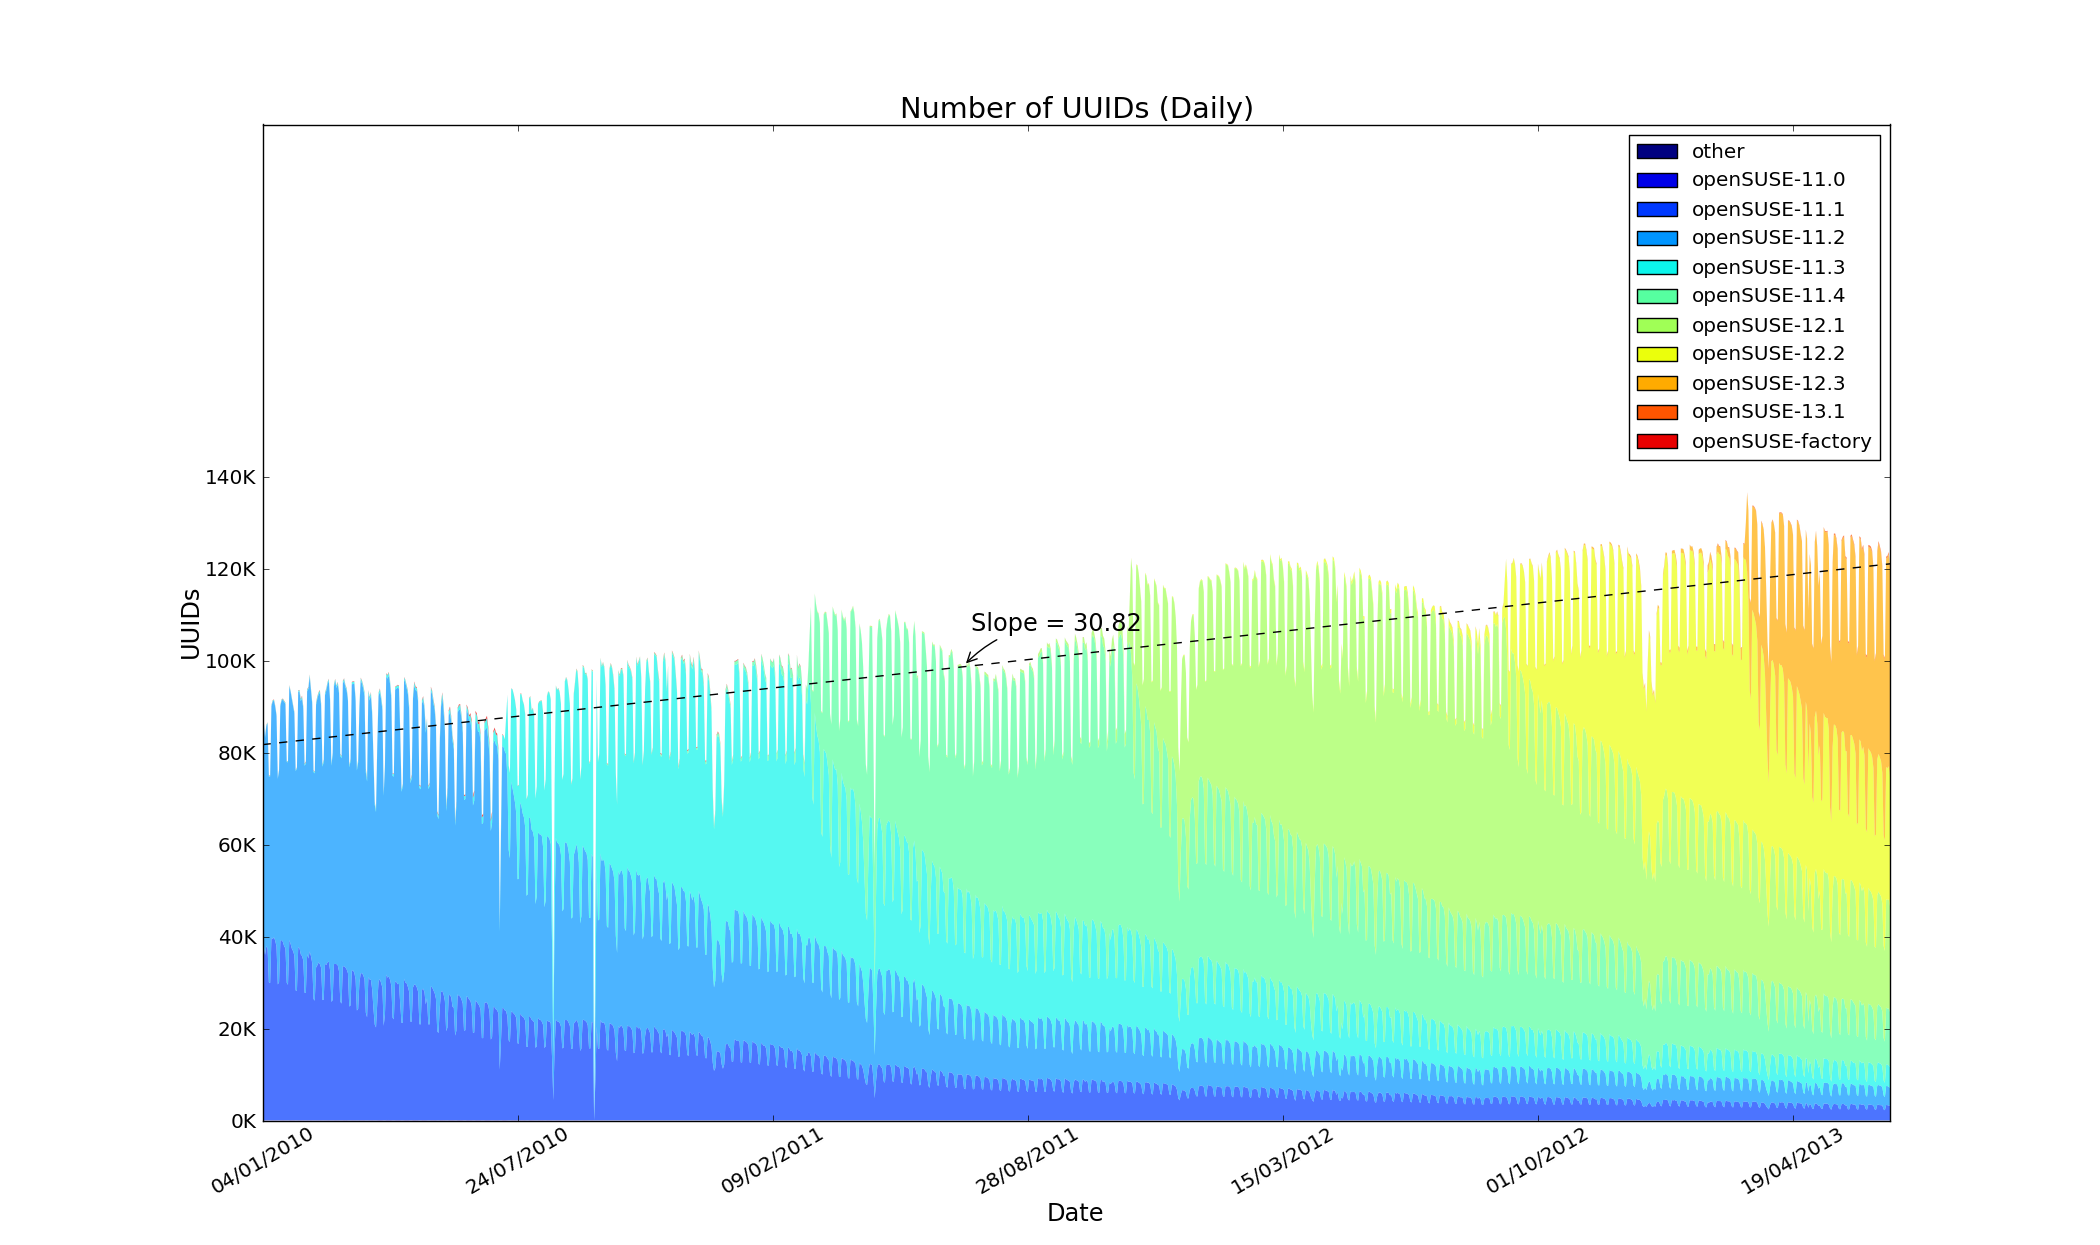
\includegraphics[height=7.2cm]{uuid_day}
\end{frame}

\begin{frame}{Weekly UUIDs}
  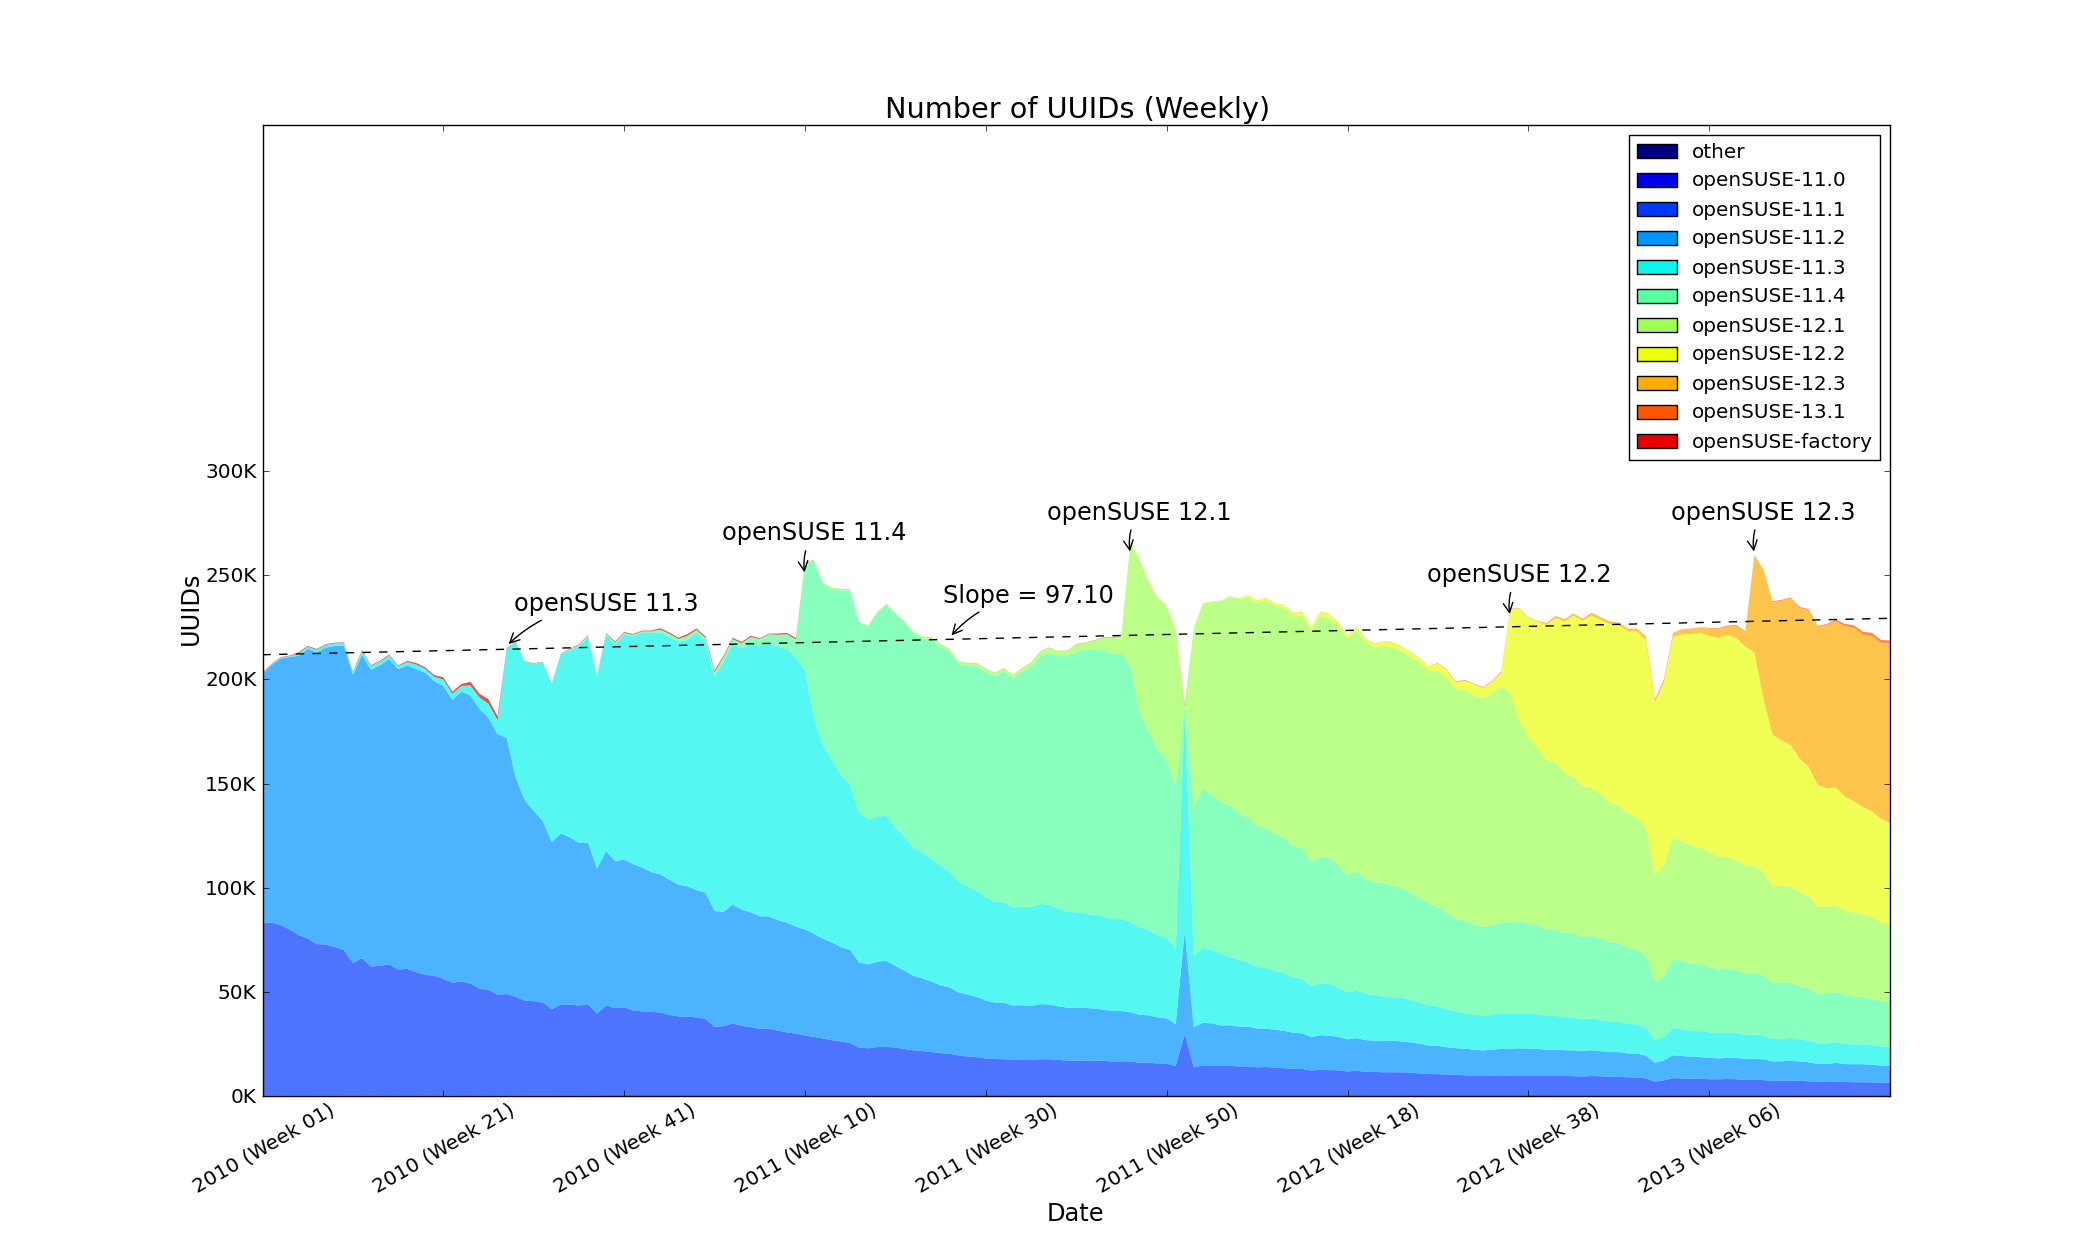
\includegraphics[height=7.2cm]{uuid_week}
\end{frame}

\begin{frame}{Monthly UUIDs}
  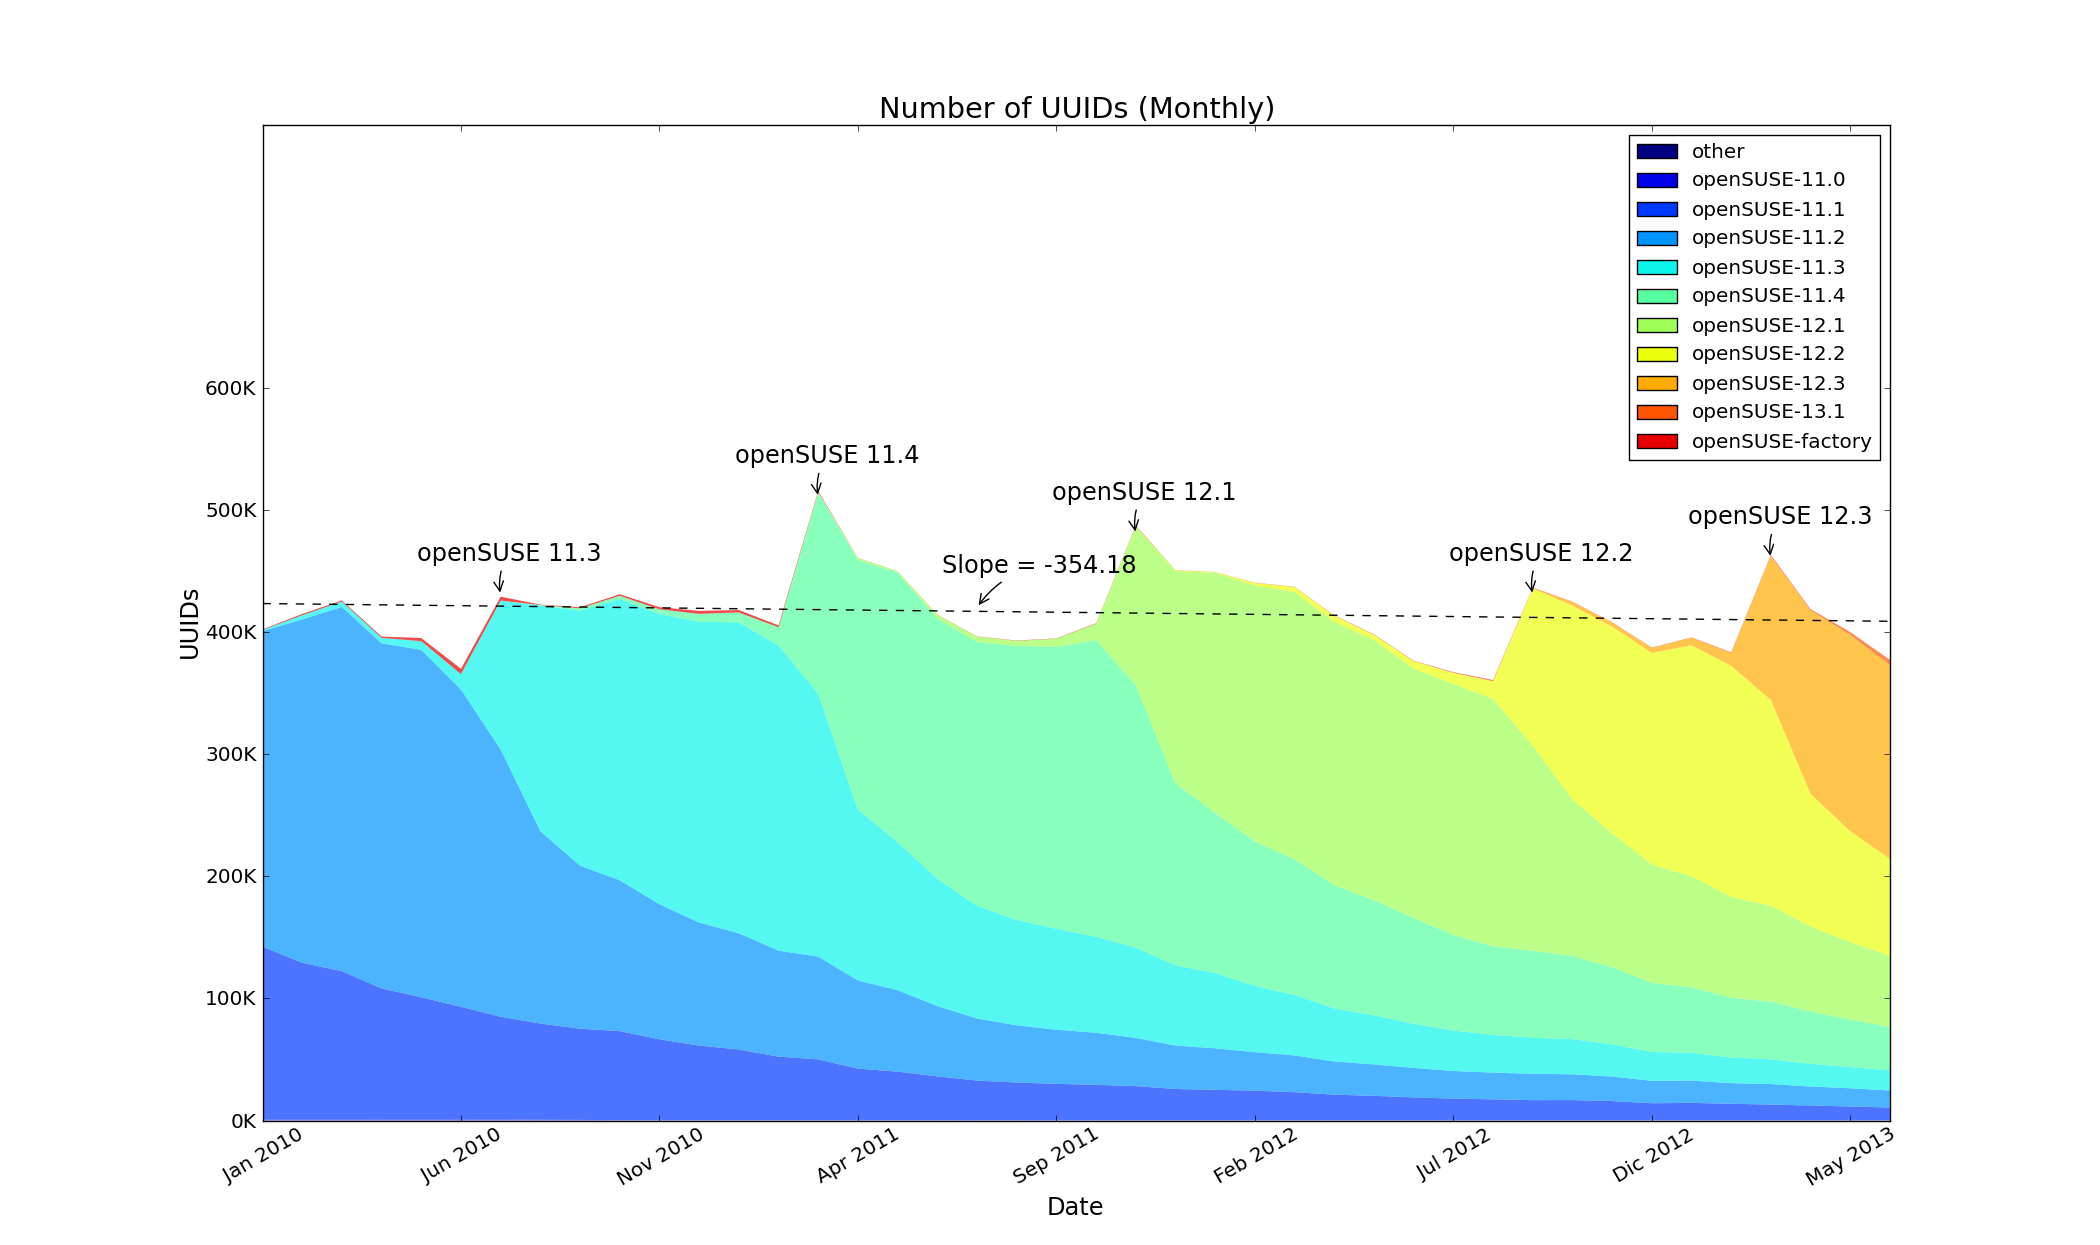
\includegraphics[height=7.2cm]{uuid_month}
\end{frame}

\begin{frame}{Users Model}
  \begin{center}
    \begin{tabular}{l r r}
      \toprule
      Date & X & Y (Users) \\
      \midrule
      01/01/2011 & 12 & 419021 \\
      01/01/2012 & 24 & 414771 \\
      01/01/2013 & 36 & 410521 \\
      01/01/2014 & 48 & 406270 \\
      \bottomrule
    \end{tabular}
  \end{center}
  \begin{itemize}
  \item Linear Model: \(y = ax + b\)
  \item Parameters: \(\left\{
    \begin{array}{l l}
      a (slope) = -354.18 \\
      b = 423271 \\
    \end{array} \right.\)
  \end{itemize}
\end{frame}


\section{Medium and Architecture}

\begin{frame}{Methodology}
  \begin{itemize}
  \item Information extracted from zypper signature
  \item Very straightforward approach: every hit is a count
  \item Caution here, they are not users, only hits
  \end{itemize}
\end{frame}

\begin{frame}{Medium and Arch}
  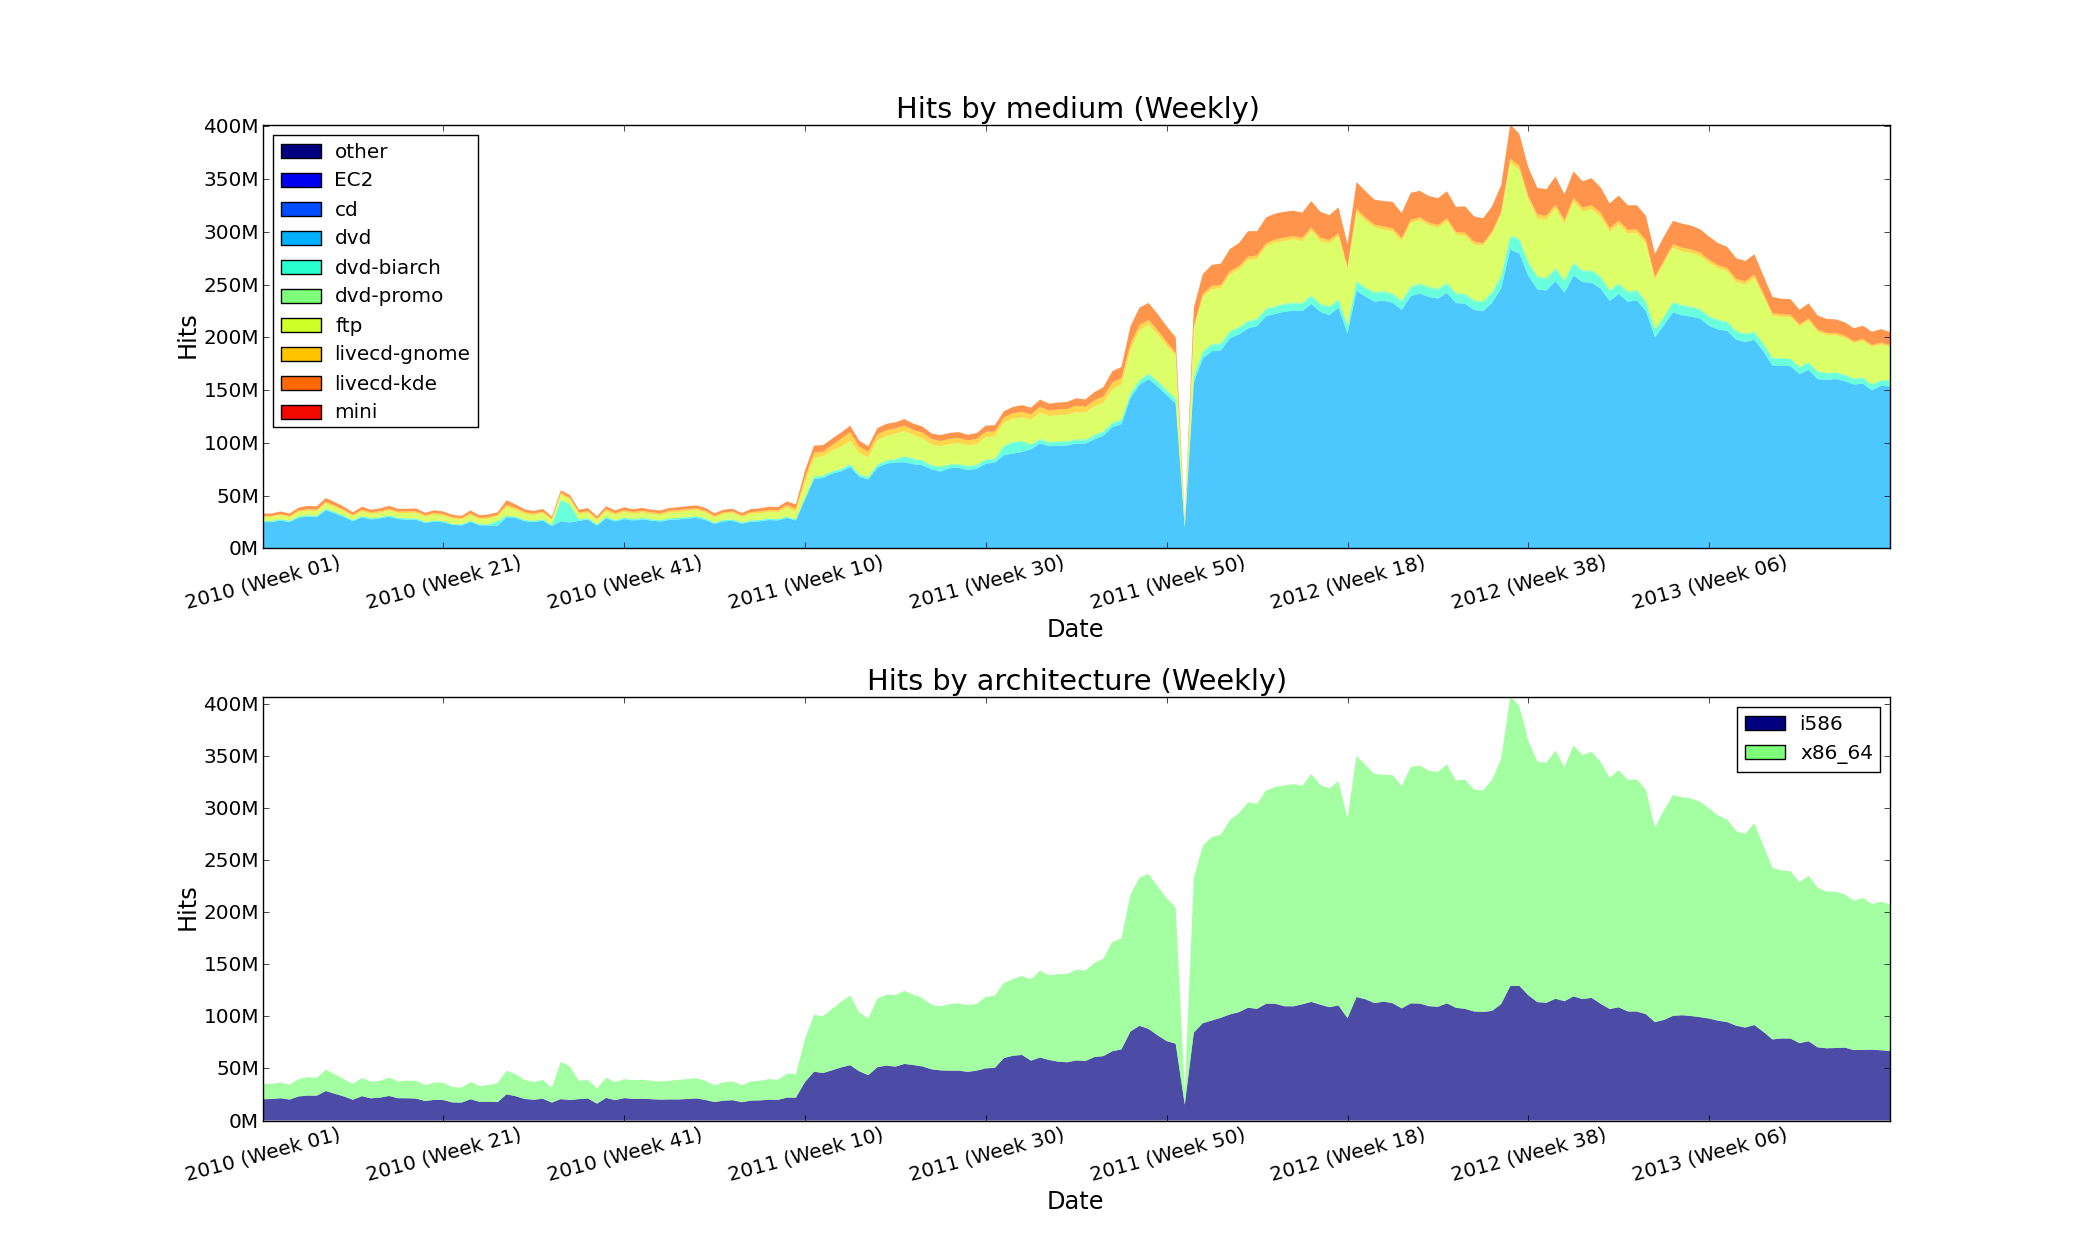
\includegraphics[height=7.2cm]{medium_arch_week}
\end{frame}


\section{Factory and Tumbleweed}

\begin{frame}{Factory and Tumbleweed - UUID count}
  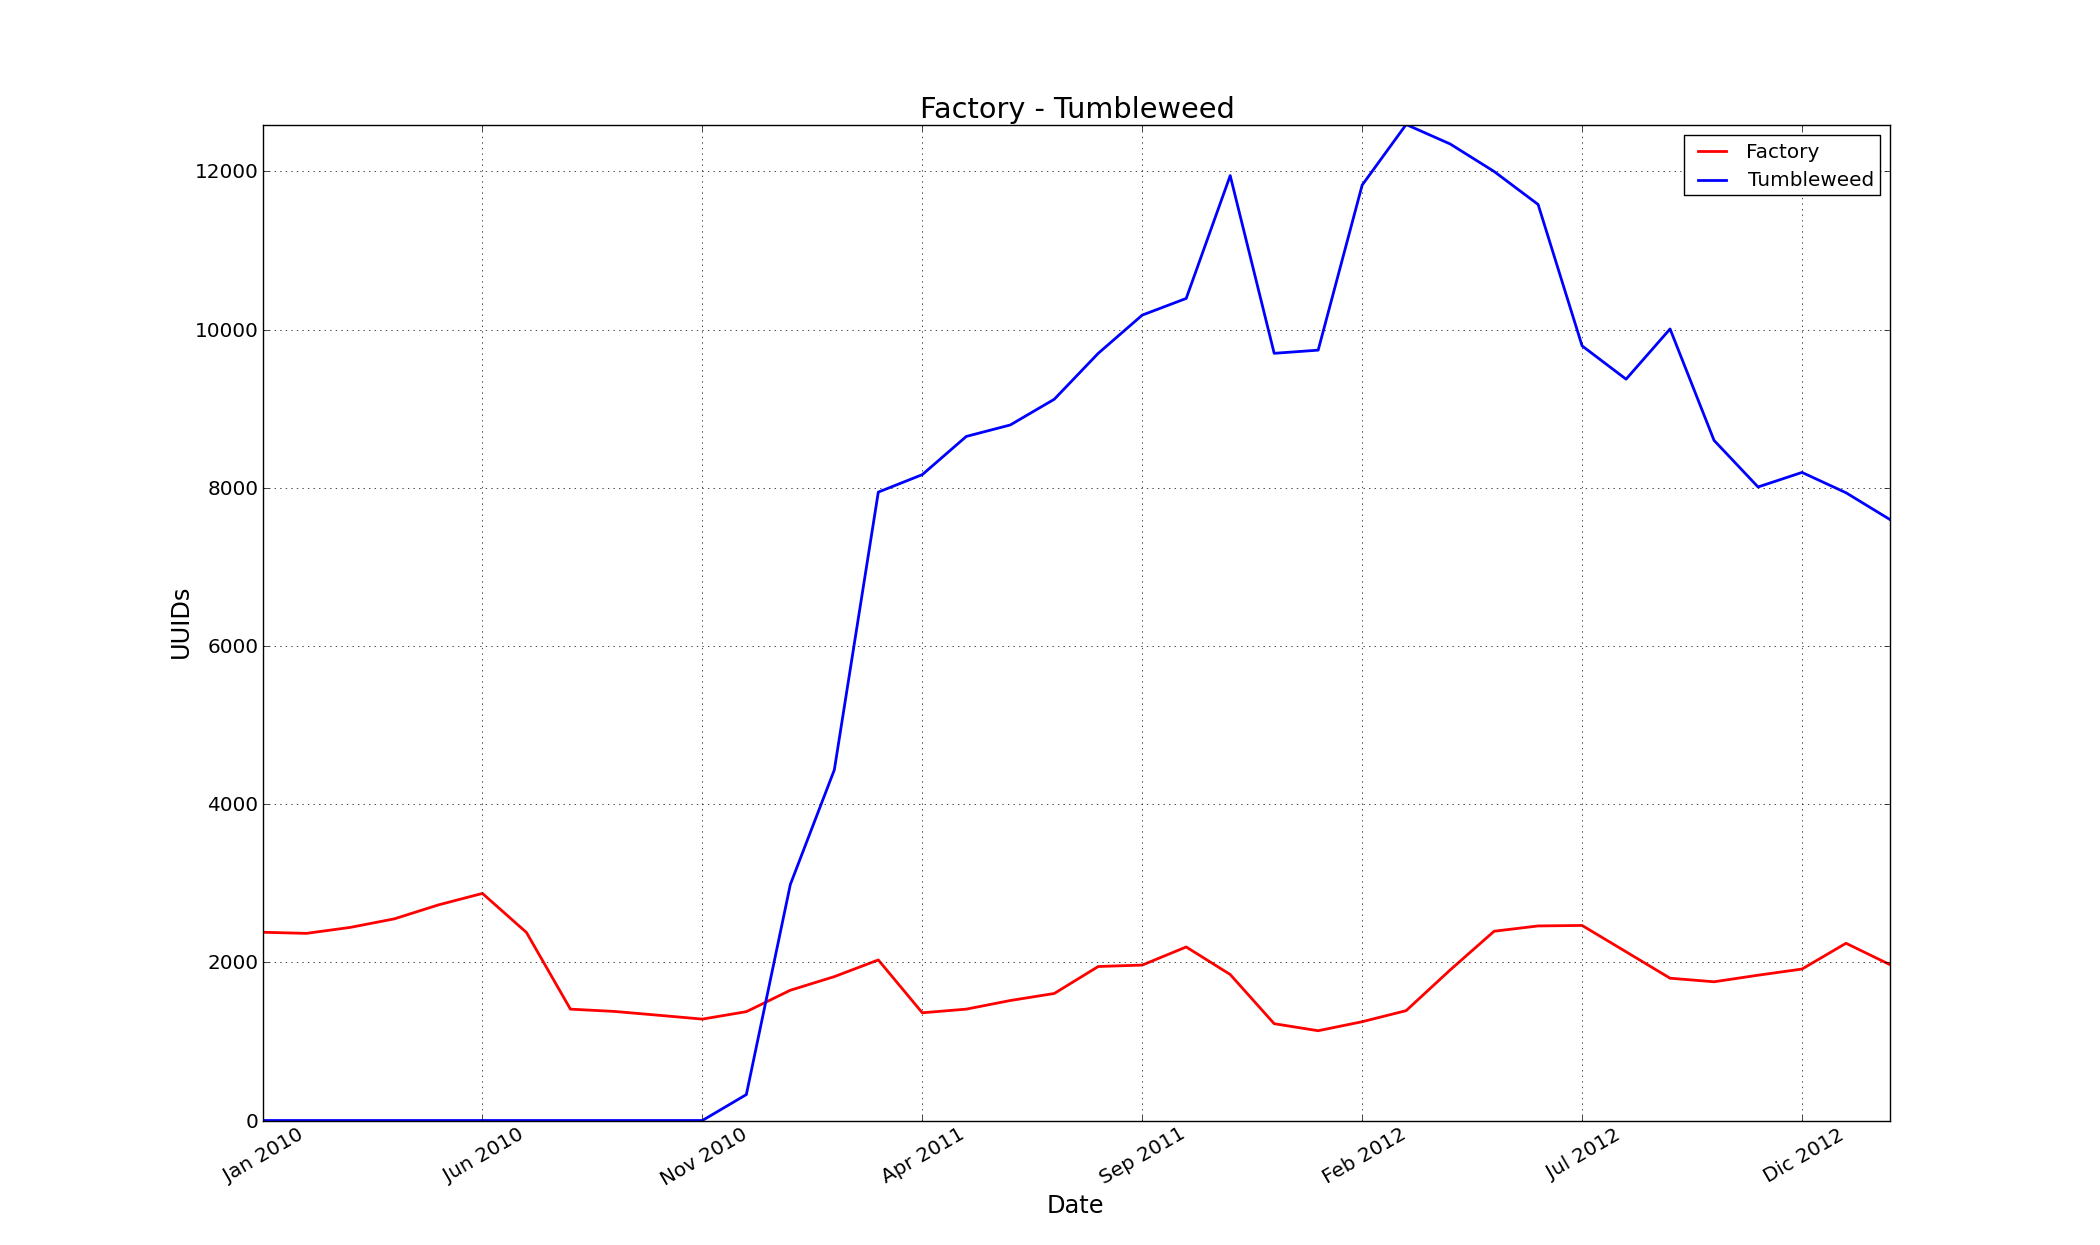
\includegraphics[height=7.2cm]{factory_tumbleweed}
\end{frame}


\section{OBS}

\begin{frame}{Methodology}
  \begin{itemize}
  \item Use the OBS API to get Submit Request (SR) list
  \item SR are to Factory and to Devel projects
  \item We are counting users in the time frame (month)
  \item Community members are identified by email
  \item Use a linear model to analyze the evolution
  \end{itemize}
\end{frame}

\begin{frame}{Submit Request (Factory and Devel)}
  \includegraphics[height=7.2cm]{obs_data}
\end{frame}

\begin{frame}{Submit Request model}
  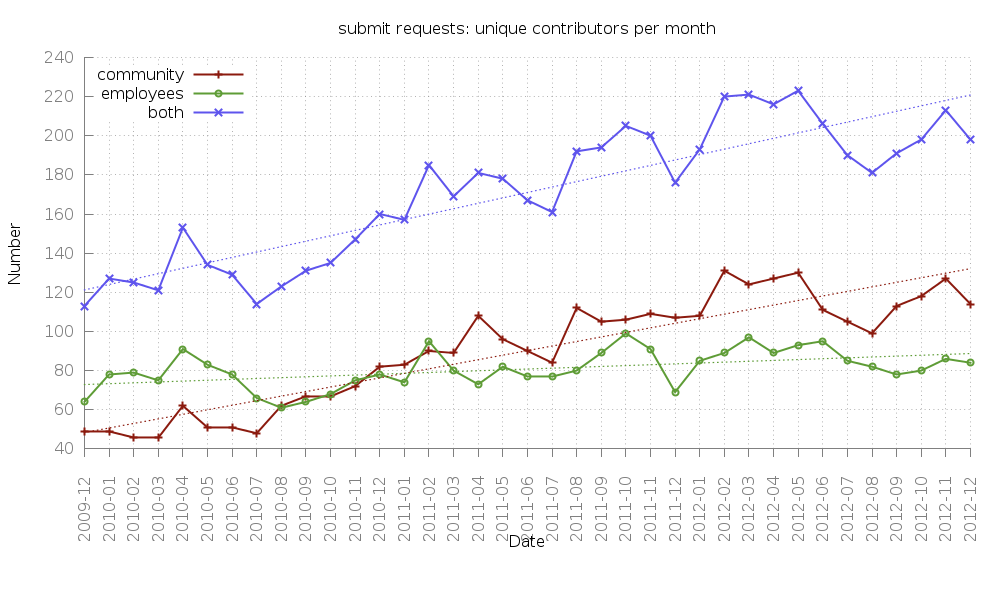
\includegraphics[height=7.2cm]{obs_model}
\end{frame}


\section{Social Media Data}

\begin{frame}{Social Media Direct Reach}
  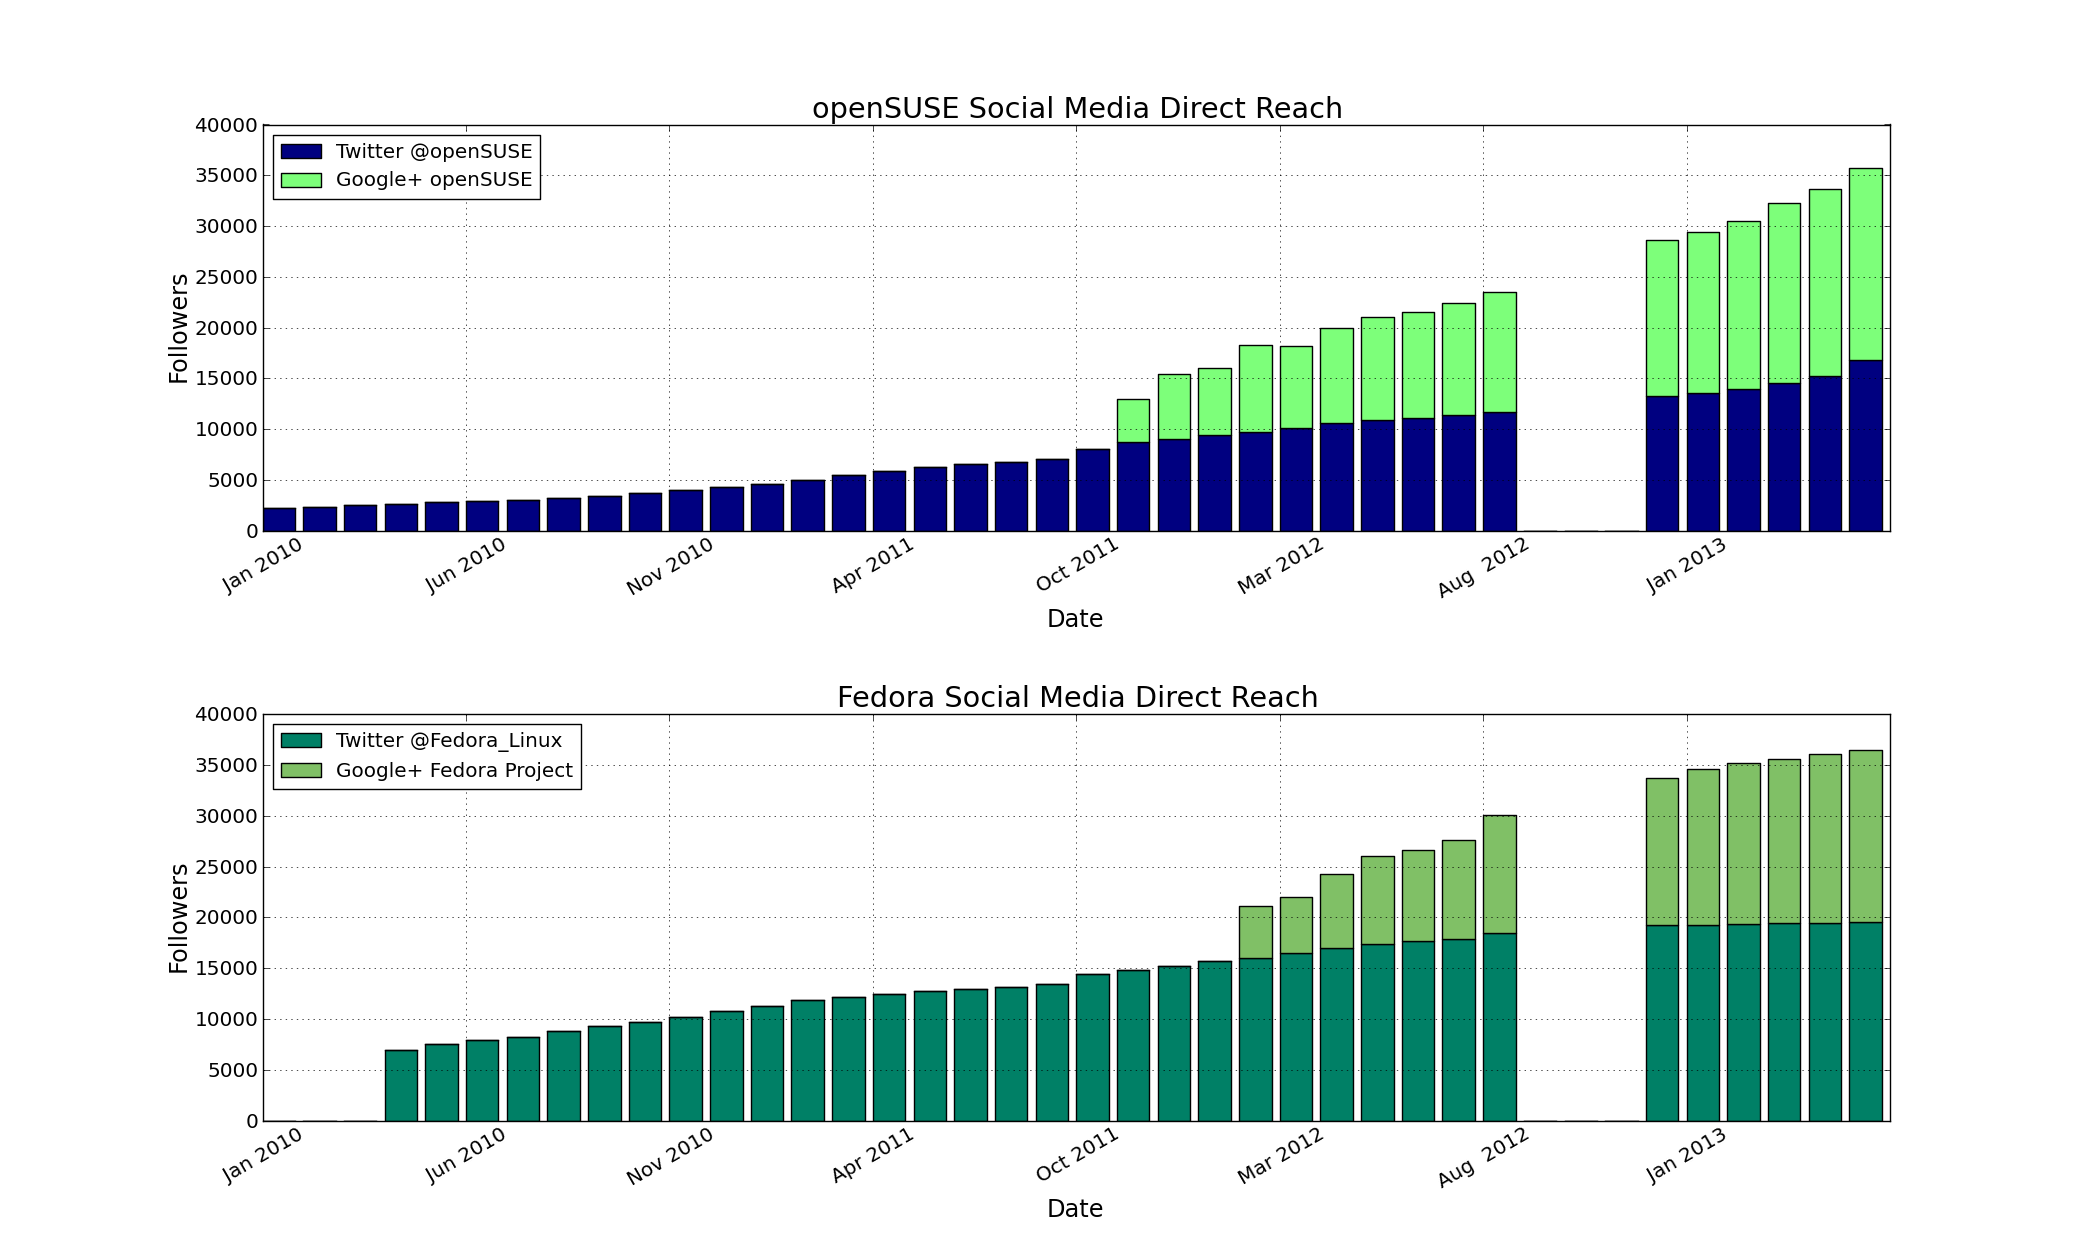
\includegraphics[height=7.2cm]{social_data}
\end{frame}


\section{openSUSE vs. Fedora}

\begin{frame}{Methodology}
  \begin{itemize}
  \item Use the same methodology that Fedora uses
  \item Scripts, data and description found in Fedora Statistics wiki \newline
        http://fedoraproject.org/wiki/Statistics
  \item Kudos for Fedora!
  \item Use new IPs never seen for this project as a basis to count users
  \item Use new IPs per day to count downloads
  \item Mangled our data to follow both rules
  \end{itemize}
\end{frame}

\begin{frame}{Reference timeline}
  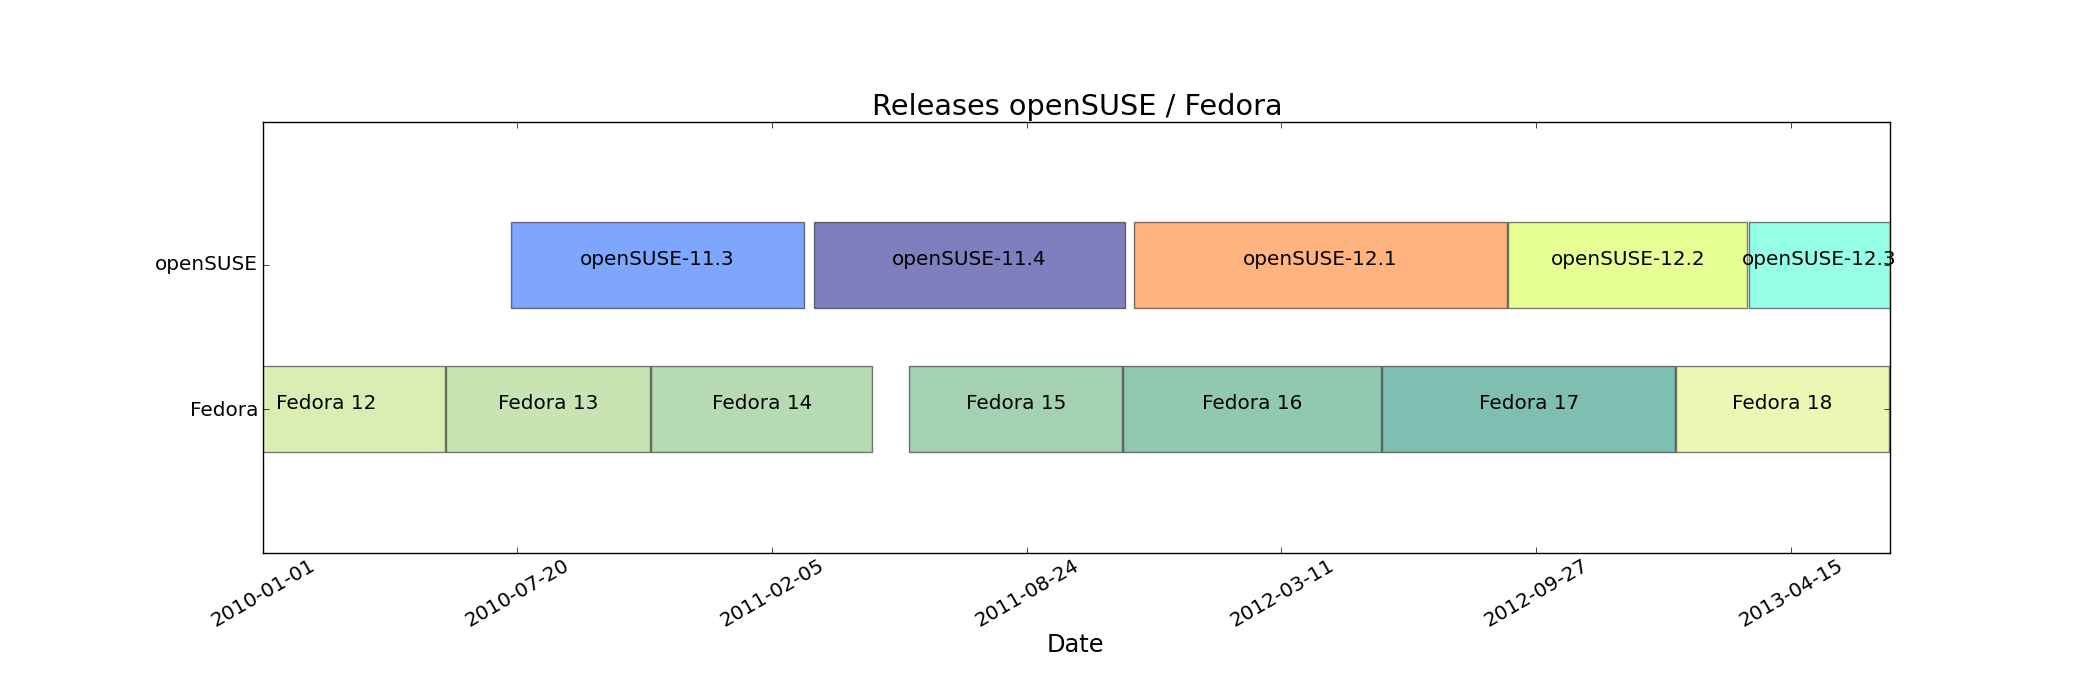
\includegraphics[height=3.6cm]{opensuse_fedora_timeline}
\end{frame}

\begin{frame}{Comparing downloads}
  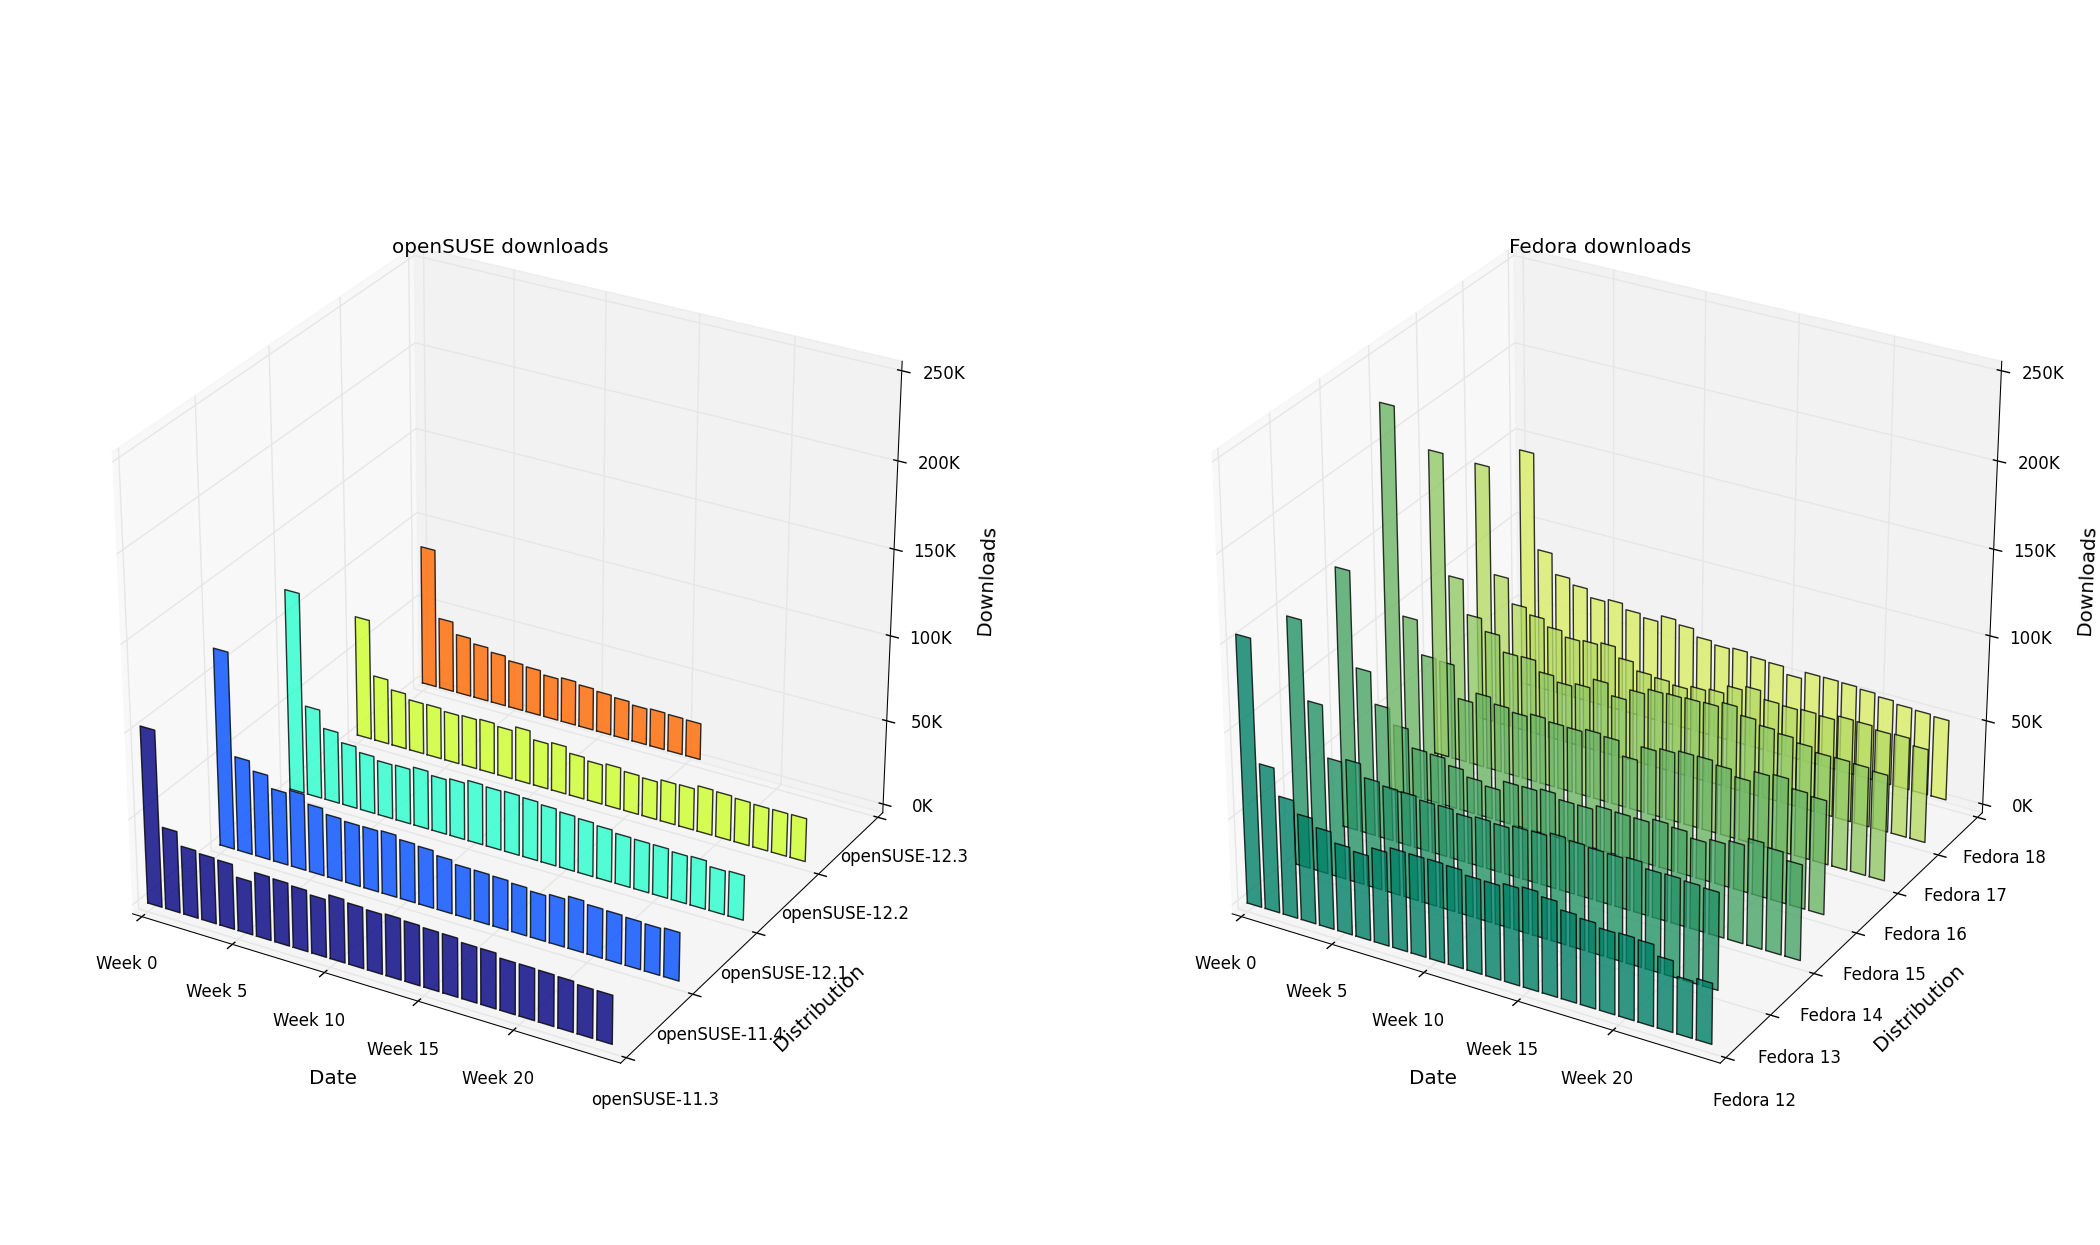
\includegraphics[height=7.2cm]{opensuse_fedora_downloads}
\end{frame}

\begin{frame}{Comparing users}
  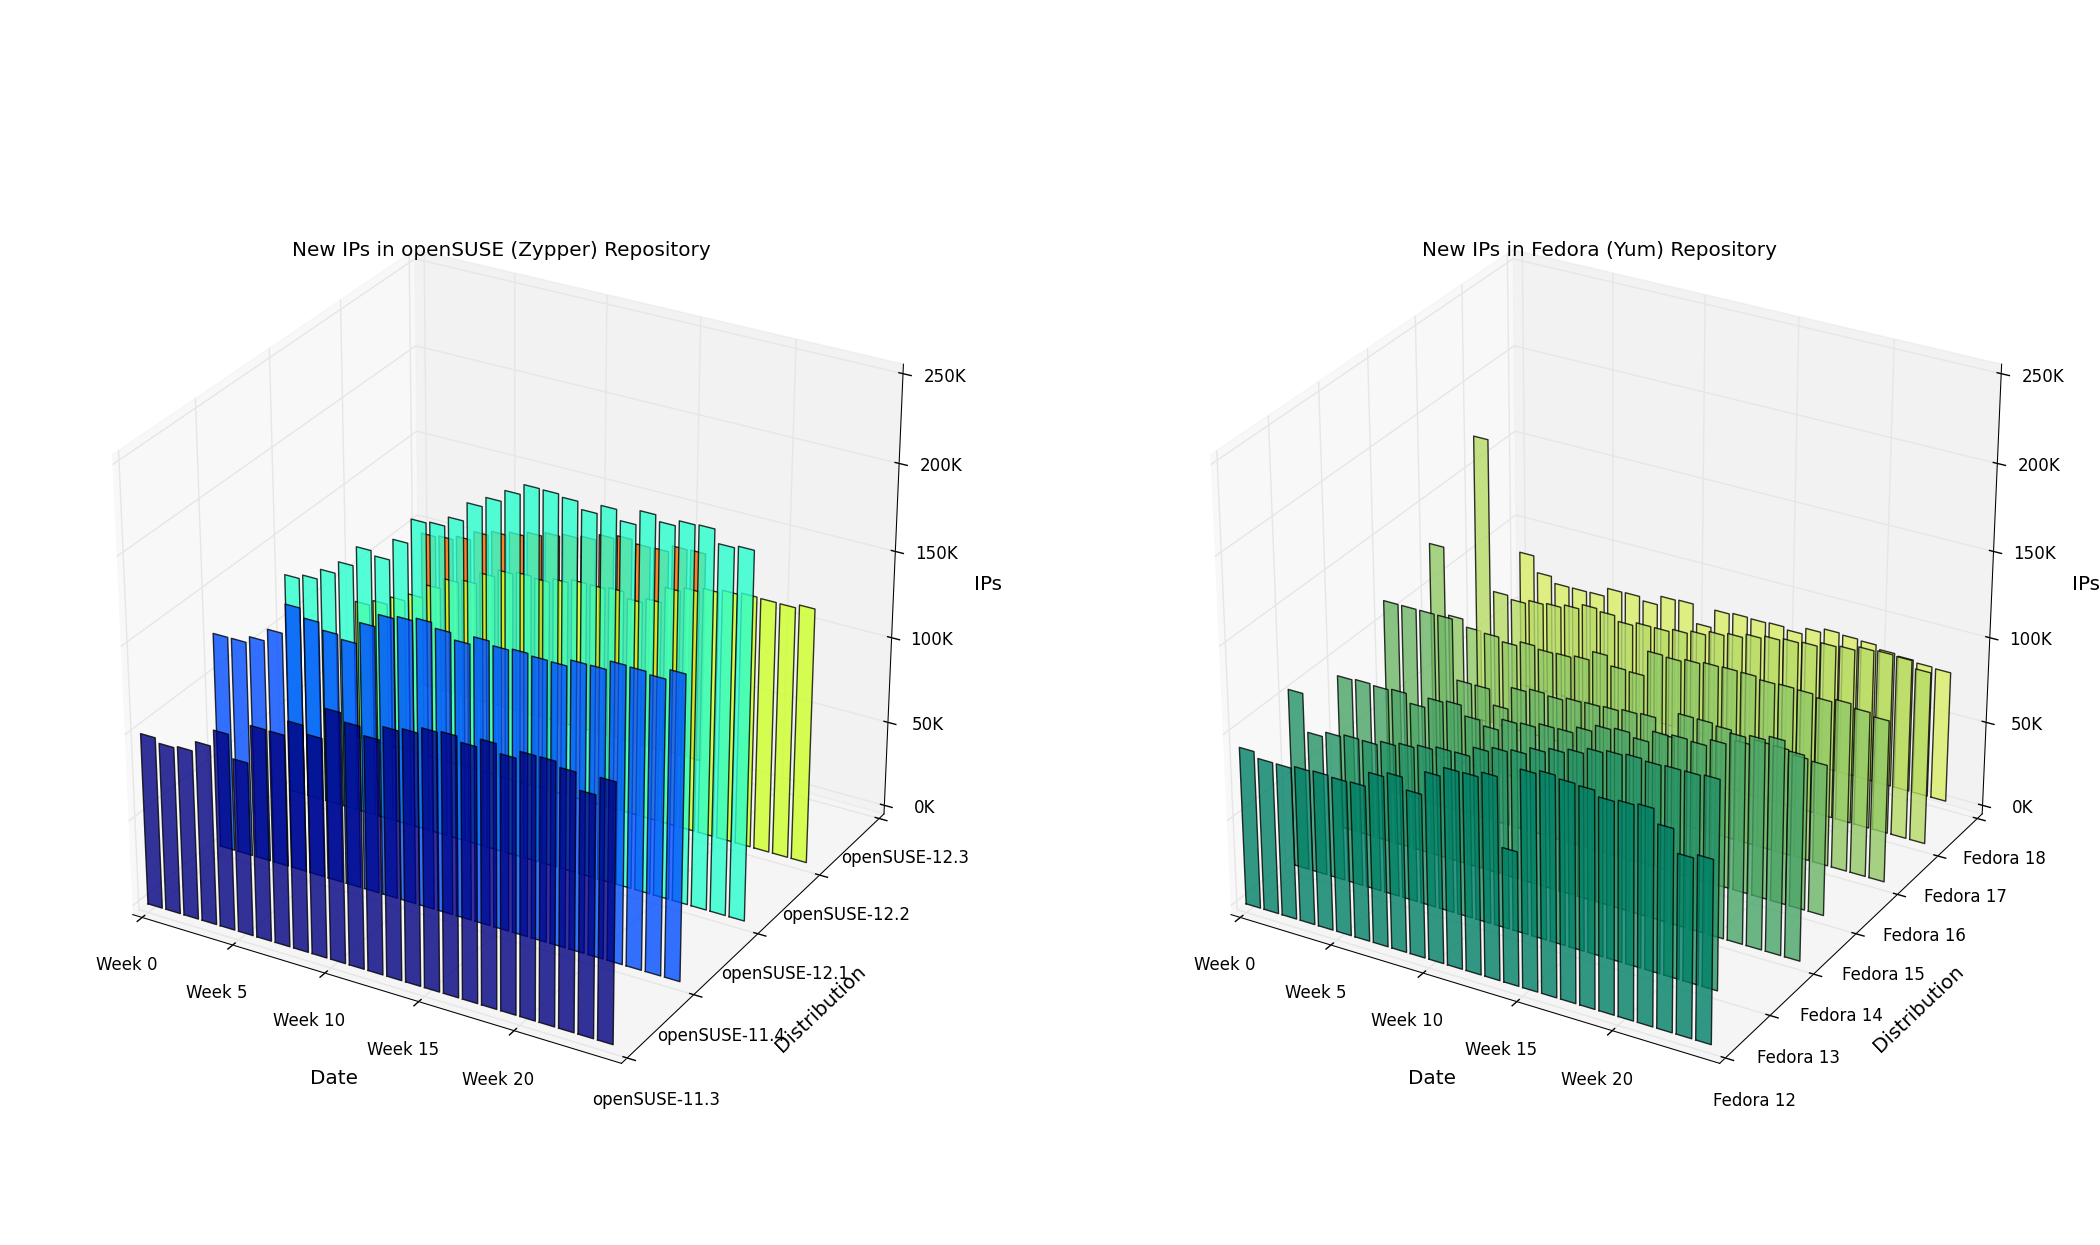
\includegraphics[height=7.2cm]{opensuse_fedora_users}
\end{frame}

\begin{frame}{Conclusion}
  \begin{center}
    \begin{huge}
      We have less downloads, but more users!
    \end{huge}
  \end{center}
  \begin{center}
    (if I didn't make a mistake)
  \end{center}
\end{frame}


\section{Endnote}

\begin{frame}{Suse is hiring}
  \begin{figure}
    
\includegraphics[width= 0.8\linewidth]{suse_hiring.png}
  \end{figure}
\end{frame}

\begin{frame}{Thanks}
  \begin{center}
    Thank you for your attention.
  \end{center}
\end{frame}

\end{document}
